

\documentclass{beamer}
 
\usepackage[utf8]{inputenc}
 \usetheme{Madrid}
 \usecolortheme{beaver}
 \usefonttheme{structuresmallcapsserif}
 \usepackage{listings}
%Information to be included in the title page:


\title[MPI] %optional
{Message Passing Interface}

\subtitle{An Overview}

\author[Dr. Joseph Kehoe] % (optional, for multiple authors)
{Joseph Kehoe\inst{1}}

\institute[IT Carlow] % (optional)
{
	\inst{1}%
	Department of Computing and Networking\\
	Institute of Technology Carlow
}

\date[ITC 2018] % (optional)
{CDD101, 2018}

\logo{
\includegraphics[height=1.5cm]{../../itcarlowlogo.png}}




 
 \AtBeginSection[]
 {
 	\begin{frame}
 		\frametitle{Table of Contents}
 		\tableofcontents[currentsection]
 	\end{frame}
 }
 
 
 
\begin{document}
 
\frame{\titlepage}
 
%  \begin{frame}
%  	\frametitle{Table of Contents}
%  	\tableofcontents
%  \end{frame}
 

    \begin{frame}
    	\frametitle{Messaging}
    	\begin{itemize}
    		\item Alternative to Procedure Calls (RPC)
    		\item More Flexibility
    		\item better suited to distributed systems
    		\item Asynchronous communication
    	\end{itemize}
    \end{frame}
  \begin{frame}
  	\frametitle{Introduction to MPI}
Message Passing Interface (MPI)
  	\begin{itemize}
  		\item Portable Message Passing Programs
  		\item Fortran,C,C++,Python, etc.
  		\item Designed for Ease of Use
  		\item Thread Safe
  		\item MPI has been standardized
  	\end{itemize}
  \end{frame}
   \begin{frame} 
    	\frametitle{Features of MPI}
    	Message Passing Interface (MPI)
    	\begin{itemize}
    		\item Point to point communications
    		\item Collective Operations
    		\item Process groups
    		\item Process Topologies
    		\item Language bindings
    	\end{itemize}
    \end{frame}

 
 
     \begin{frame}
     	\frametitle{Tutorial Code}
     	\begin{itemize}
     		\item We will follow the MPI tutorial \href{https://github.com/wesleykendall/mpitutorial}{here}
     		\item Download the tutorial and compile the code (I assume you will be using unix)
     	\end{itemize}

     \end{frame}
     
          \begin{frame}
          	\frametitle{Hello World}
          	\begin{itemize}
          		\item Initiialise MPI with:
          		\item \texttt{MPI\_Init(NULL, NULL);}
          		\item Get number of processes with:
          		\item \texttt{MPI\_Comm\_size(MPI\_COMM\_WORLD, \&world\_size);}
          		\item Get our rank with:
          		\item \texttt{MPI\_Comm\_rank(MPI\_COMM\_WORLD, \&world\_rank);}
				\item End program with:
				\item  \texttt{MPI\_Finalize();}
          	\end{itemize}
        \end{frame}
        \begin{frame}[fragile=singleslide]
        	\frametitle{Sending and Receiving}  	
          	  \begin{verbatim}
int number;
if (world_rank == 0) {
    number = -1;
    MPI_Send(&number, 1, MPI_INT, 1, 0, MPI_COMM_WORLD);
} else if (world_rank == 1) {
    MPI_Recv(&number, 1, MPI_INT, 0, 0, 
              MPI_COMM_WORLD, MPI_STATUS_IGNORE); 
    printf("Process 1 received  %d from process 0\n", number); 	  
}
          	  \end{verbatim} 
         \end{frame}
         \begin{frame}
         	\frametitle{Message Parameters of Send}
         	\begin{itemize}
         		\item Address of start of data being sent
         		\item Number of items of data being sent 
         		\item Type of data
         		\item Rank of destination
         		\item Message Tag (integer)
         		\item Communicator (handle)
         	\end{itemize}
         
         \end{frame}   
                  \begin{frame}
                  	\frametitle{Message Parameters of Receive}
                  	\begin{itemize}
                  		\item Address of start of receiving buffer
                  		\item Number of items of data being received 
                  		\item Type of data
                  		\item Rank of source
                  		\item Message Tag (integer)
                  		\item Communicator (handle)
                  		\item A status object
                  	\end{itemize}
                  	
                  \end{frame} 
      \begin{frame}
      	\frametitle{MPI Primitives}
      	\begin{description}
      		\item[MPI\_bsend] Append outgoing message to local send buffer
      		\item[MPI\_send] Send a message and wait until copied to local or remote buffer
      		\item[MPI\_ssend] Send a message and wait until receipt starts
      		\item[MPI\_sendrecv] Send a message and wait for reply
      	\end{description}
      	%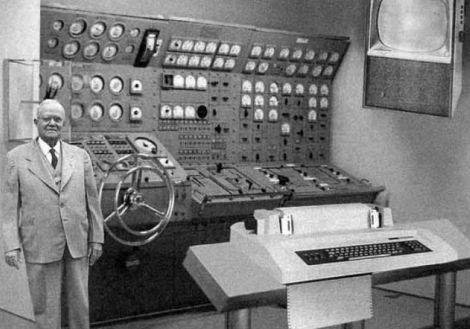
\includegraphics[height=4cm]{Old-Server.jpg}
      \end{frame}
      \begin{frame}
      	\frametitle{MPI Primitives}
      	\begin{description}
      		\item[MPI\_isend] Pass reference to outgoing message, and continue
      		\item[MPI\_issend] Pass refence to outgoing message , and wait until receipt starts
      		\item[MPI\_recv] Receive a message, block if there is none
      		\item[MPI\_irecv] Check if there is an incoming message, but do not block
      	\end{description}
      	\href{http://materials.jeremybejarano.com/MPIwithPython/introMPI.html}{see here}
      	%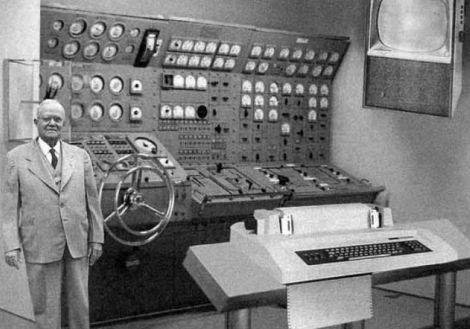
\includegraphics[height=4cm]{Old-Server.jpg}
      \end{frame} 


        
\end{document}

